\chapter{Overview of OMR}
\label{c:overveiw-of-omr}

In this section, previous works of OMR are mentioned. Preprocessing (binarization, staff profiling, staff detection, and staff removal) and recognition (symbol segmentation, symbol classification) are included. 

\section{Binarization}
% Binarization

% \begin{figure}[ht]
%     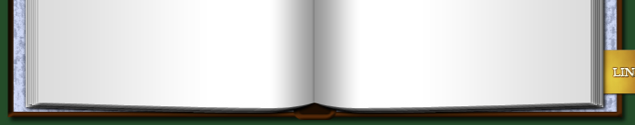
\includegraphics[width=\textwidth]{bookspine}
%     \caption{Example of the gray-scale image near the book spine\label{fig:bookspine}.}
% \end{figure}

\section{Staff Detection and Removal}

% Dalitz et al.~\cite{Dalitz:2008:CSoSRA} introduced a systematic way for testing the staff removal algorithms. A dataset was generated from a set of ideal score images with the deformation methods listed in Table.~\ref{table:deformation}. The deformation algorithms and the CVC-MUSCIMA dataset are made openly available by Forns et al.~\cite{Forns:2012:CVC-MUSCIMA}.

% \begin{table}[ht]
%     \hspace{-.5in}
%     \begin{tabular}{|c|c|c|}
%         \hline
%         {\bf Deformation} & {\bf Type} & {\bf Parameter Description} \\
%         \hline
%         Curvature & deterministic & height/width ratio of sine curve \\
%         \hline
%         Typeset Emulation & both & \parbox[c]{9cm}{gap width, maximal height and variance of vertical shift} \\
%         \hline
%         Line Interruptions & random & \parbox[c]{9cm}{interruption frequency, maximal width and variance of gap width} \\
%         \hline
%         Thickness Variation & random & \parbox[c]{9cm}{Markov chain stationary distribution and inertia factor} \\
%         \hline
%         $y$-variation & random & \parbox[c]{9cm}{Markov chain stationary distribution and inertia factor} \\
%         \hline
%         Degradation & random & \parbox[c]{9cm}{emulating local distortions suggested by Kanungo et al.~\cite{Kanungo:2000:Degradation}} \\
%         \hline
%         White Speckles & random & \parbox[c]{9cm}{speckle frequency, random walk length and smoothing factor} \\
%         \hline
%     \end{tabular}
%     \caption{Deformation Methods\label{table:deformation}.}
% \end{table}
